\documentclass{article}

\usepackage{graphicx}
\usepackage{hyperref}
\usepackage{url}

\author{ The B.O.M. \\
\small{The Ball Of Mud}\\
\small{Omar Pakker, Chiel Peters, Mary Gouseti, Cindy Berghuizen}}
\title{Reputation management for airline companies}

\begin{document}
\maketitle

\section*{Introduction}

There are currently many outlets on which customers can leave feedback about the quality of an airline: tripadvisor, booking.com, twitter or any social network site where people can post reviews. However these reviews are scattered across the internet. This makes analysis hard for clients, airline companies and other users. Therefore a new system is being developed that collect all the different reviews together.

The purpose of this document is to research the different possibilities of the system's architecture. Section two contains the key quality attributes of the system. In section three the use cases are stated and explained. Finally in section four the solution proposal for the architecture is given.

\section*{Key quality attributes}

In order to build the architecture first the key quality attributes need to be stated. The quality attributes question how the key components of the system should behave. No answers are given in this section however it points out the main questions which aid in the design and trade-offs later.

\subsection*{Availability}
Availability is one of the key factors for the clients such as airline companies. The system should be build according to their needs. Therefore a important question is: How does the system reach the end users?

\subsection*{Scalability}
The amount of data gathered by the system is quite a lot. The system should be able to efficiently store and handle this data. 
For now it is unknown how many users will make use of this review system. However in order for the system to be a success it should be accessible to a high amount of users. Therefore trade-offs need to be made related the following questions:

\begin{itemize}
\item How much resources need to be allocated in order to keep our system up to date with the external sources?
\item How many active users should the system be able to handle at the same time?
\item How will our system access the external data-sources and what will we do with it?
\item What kind of (temporary) storage for the rapidly changing data is needed, if any is needed.
\end{itemize}

\subsection*{Modifiability}
The system is depending on external sources. Those external sources are part of the ever changing internet. Also, our stakeholders will have a wide variety of needs which may change over time. The important questions about this are:

\begin{itemize}
\item How can our system cope with changes in external data sources?  
\begin{itemize}
\item What if another external data-source has to be added or an external data-source changes it's structure?
\end{itemize}
\item How can we modularize our system to keep changes from stakeholders maintainable?
\end{itemize}

\section*{Scenario Analysis}

The most important questions from the attribute are: 
\begin{itemize}
\item How much resources need to be allocated in order to keep our system up to date with the external sources?
\item What kind of (temporary) storage for the rapidly changing data is needed?
\item How will our system access the external data-sources?
\end{itemize}

In order to answer these questions first an overall figure of the system is given in Figure \ref{fig:fig1}. 
Throughout an interface the user will request for data (e.g. airline information). Then the purpose of the system is to gather
the data and show the data to the user in a given format. The process of data gathering is the key attribute of this system.
In this document three different data gathering processes are explored:

\begin{figure}[!]
\centering
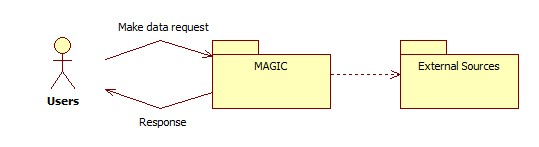
\includegraphics[width=300px]{UserRequestingData}
\caption{Overall use case}
\label{fig:fig1}
\end{figure}

\begin{enumerate}
\item Immediate request: No storage is allocated and the request is forwarded to all external sources immediately. This process is depicted in Figure \ref{fig:fig2}.  

\begin{figure}[!htbp]
\centering
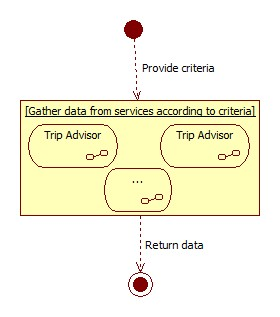
\includegraphics[width=200px]{Realtime}
\caption{Real time requesting of the airline reviews}
\label{fig:fig2}
\end{figure}

\item Global polling: The data from the external sources (twitter, tripadvisor, etc.) is stored in a separate database. A polling mechanism is put in place to synchronize the database with the external sources. One mechanism/process exists to update the external sources in a sequence. Data request from users will result on request on the database. This process is depicted in Figure \ref{fig:fig3}.  
\item Independent polling: The data is stored from the external sources into a
separate database. However instead of one process polling the external sources
these can be separated. For example some sources change more frequently than
others therefore it makes sense to poll at different time mechanism's. Data
request from users will result on request on the database. This process is
depicted in Figure \ref{fig:fig4}.  
\end{enumerate}

\begin{figure}[!]
\centering
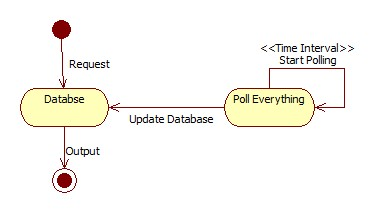
\includegraphics[width=300px]{GlobalPolling}
\caption{Global polling of the external resources to a database}
\label{fig:fig3}
\end{figure}

\begin{figure}[!]
\centering
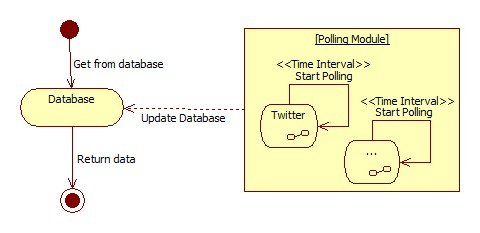
\includegraphics[width=300px]{IndependentPolling}
\caption{Independent polling of the external resources to a database}
\label{fig:fig4}
\end{figure}

Although the real time architecture would be ideal towards the clients, it is however not feasible within the scalability quality attribute. As this would require non-stop forwarding and collecting data requests from the external sources and would lead to a high amount of bandwidth. Therefore to avoid non-stop polling of the same data a database was added. However this also introduces problems related to keeping the database up to date. The database can be updated from the external sources by a polling mechanism. A global polling mechanism would be the most simple solution however this does not account for the differences between the external sources. For instance, twitter is more volatile than tripadvisor. Hence an independent polling mechanism would be more appropriate as it can account for these differences and can also occur asynchronously. 
Independent polling also enhances the modifiability of the software.
A small polling module for a new data-source can be added instead of making larger changes in the module layer. Also, when an external data-source changes we can modify the module it is linked to.

One big company utilizing a system similar to the above polling is Google. Google utilizes a crawler to scan the web and store relevant data. Papers /cite{GFD} and /cite{Dremel} describe how Google then handles and searches this data.

Getting data from the database to the user can also be done in different ways
\begin{enumerate}
\item Send a request to the database which will return the data
\item Send a request to a cache, which will see if the data is still (partly) in the cache. If the data is present it will check it's validity. When the data is not in the cache or has become invalid, the data will be gathered from the database and stored in the cache.  This procedure be seen in Figure \ref{fig:fig5}
\end{enumerate}

\begin{figure}[!]
\centering
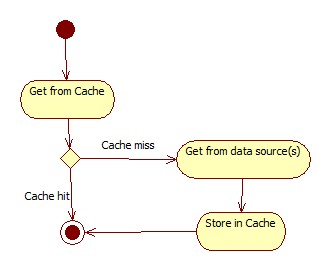
\includegraphics[width=200px]{Cached}
\caption{Cache structure}
\label{fig:fig5}
\end{figure}

Since there will be a lot of data present in the database, searching through the database can be a slow process. The cache structure will speed up the searching process if the data is already present in the cache. There are numerous ways to handle caching. A paper by Yahoo /cite{Yahoo} shows numerous measurements and comparisons.
\section*{Architecture proposal}

In order to answer the questions concerning the key quality attributes we propose the architecture presented in Figure \ref{fig:fig6}.

%With the findings of the previous section we propose the solution shown in Figure \ref{fig:fig6}.

The proposed architecture consists of separate layers to increase
modifiability and maintainability. For instance, the GUI and the Business Logic
are separated. As a result of this, when the GUI has to change it will have no effect on
the rest of the program; this will make it easy to a add a new interface e.g.
a mobile interface. The Business Logic layer will handle all the requests from
the GUI layer by processing the input and output data.
This is a popular design and is for instance used as the base architecture in Chapter 2 of \cite{MSDN}.

From the Business Logic Layer the request will be directed to the
Cache. If there are parts of the data in the cache it will check if the data is
still valid using one of the algorithms currently available for cache
invalidation. If the data is not valid or the data is not in the Cache the
request is directed to the database. By using a Cache and reducing the number
of requests sent to the database we reduce the workload and achieve better
performance and scalability.

In order to gather data the database is connected to a polling module. The
polling module will handle the polling of the data from the external sources.
The polling module consists of different smaller modules. This is done to increase the maintainability and modifiability.
Each module is optimised to harvest data from a specific external source according to its
characteristics. Additionally, the Data Access Layer will be responsible for transforming the
harvested data's universal format, e.g. xml, JSON etc, and updating the database when the data has changed.

\begin{figure}[!]
\centering
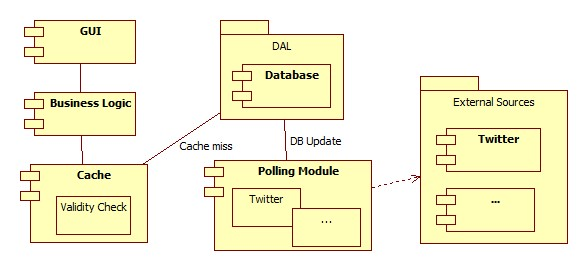
\includegraphics[width=300px]{ProposedSolution}
\caption{Architecture proposal}
\label{fig:fig6}
\end{figure}


\newpage

\nocite{*}
\bibliographystyle{amsplain}
\bibliography{mybib}
\end{document}